\documentclass{sig-alternate}

% UTF8 support
\usepackage[utf8x]{inputenc}


\usepackage{hyperref}
\usepackage{epsf,graphicx}
\graphicspath{{figures/}}
\usepackage{multicol}
\usepackage{subcaption}
\usepackage{booktabs}

\usepackage[usenames,dvipsnames]{xcolor}
\usepackage{tikz}
\usetikzlibrary{positioning, calc}

\usepackage[draft,nomargin,footnote]{fixme}

\newcommand{\eg}{{\textit{e.g.~}}}
\newcommand{\etal}{{\textit{et al.~}}}
\newcommand{\ie}{{\textit{i.e.~}}}

% for mutual modelling in CSCL
\newcommand{\M}[3]{{\mathcal{M}(#1, #2, #3)}}
\newcommand{\model}[3]{{$\mathcal{M}(#1, #2, #3)$}}
\newcommand{\Model}[3]{{$\mathcal{M}^{\circ}(#1, #2, #3)$}}

\newcommand{\refmodel}[2]{{$\mathcal{M}(#1, #2)$}}

\newcommand{\groundingcriterion}{{$\mathcal{M}^{\circ}_{min}$}}
\newcommand{\inigrounding}{{$\mathcal{M}^{\circ}_{t_0}$}}



%
% --- Author Metadata here ---
\conferenceinfo{10th ACM/IEEE International Conference on Human-Robot Interaction}{2015 Portland, USA}
%\CopyrightYear{2007} % Allows default copyright year (20XX) to be over-ridden - IF NEED BE.
%\crdata{0-12345-67-8/90/01}  % Allows default copyright data (0-89791-88-6/97/05) to be over-ridden - IF NEED BE.
% --- End of Author Metadata ---

%(DH) is it too soon to claim learning by teaching benefits in the title...? 
%(DH) the paper is not about "learning handwriting", it's about the robot.
\title{\LARGE \bf
Mutual Modelling in Robotics: \\Inspirations for the Next Steps
}

% \numberofauthors{3} 
% \author{
% \alignauthor
% Séverin Lemaignan\\
% Pierre Dillenbourg\\
%    \affaddr{Computer-Human Interaction in Learning and Instruction Laboratory (CHILI)}\\
%    \affaddr{École Polytechnique Fédérale\\ de Lausanne (EPFL)}\\
%    \affaddr{CH-1015 Lausanne, Switzerland}\\
%    \email{firstname.lastname@epfl.ch}
% \alignauthor
% Claire Braboszcz\\
%    \affaddr{Laboratory for Neurology \& \\Imaging of Cognition (LabNIC)}\\
%    \affaddr{University of Geneva}\\
%    \affaddr{CH-1211 Geneva, Switzerland}\\
%    \email{claire.braboszcz@unige.ch}
% }

%(DH) my EPFL email address won't work for much longer....


\begin{document}

\maketitle

%%%%%%%%%%%%%%%%%%%%%%%%%%%%%%%%%%%%%%%%%%%%%%%%%%%%%%%%%%%%%%%%%%%%%%%%%%%%%%%%
\begin{abstract}

Mutual modelling, the reciprocal ability to establish a mental model of the
other, plays a fundamental role in human interactions. This complex cognitive
skill is however difficult to fully apprehend as it encompasses multiple
neuronal, psychological and social mechanisms that are generally not easily
turned into computational models suitable for robots.

This article presents several perspectives on mutual modelling from a range of
disciplines, and reflects on how these perspectives can be beneficial to the
advancement of social cognition in robotics. We gather here both basic tools
(concepts, formalisms, models) and exemplary experimental settings and methods
that are of relevance to robotics.

This contribution is expected to consolidate the corpus of knowledge readily
available to human-robot interaction research, and to foster interest for this
fundamentally cross-disciplinary field.

\end{abstract}


%%%%%%%%%%%%%%%%%%%%%%%%%%%%%%%%%%%%%%%%%%%%%%%%%%%%%%%%%%%%%%%%%%%%%%%%%%%%%%%%
\section{Introduction}

Human social dynamics rely upon the ability to effectively attribute beliefs,
goals and percepts to other people. This set of meta-representational abilities
shapes what is called a theory of mind (ToM) or the ability to mentalize, and leads to
mutual modelling: the reciprocal ability to establish a mental model of the
other. This lays at the core of human interactions: normal human social
interactions depend upon the recognition of other sensory perspectives, the
understanding of other mental states, and the recognition of complex non-verbal
cues of attention and emotional state.

As such, adapting and transferring these cognitive skills to social robots is an important
research objective.

Until now, however, the human-robot interaction (HRI) community has only
scratched the surface: in~\cite{scassellati2002theory}, Brian Scassellati gave
an initial account of Leslie's and Baron-Cohen's respective models of the
emergence of a theory of mind (we discuss them below) from the perspective of
robotics, but reported implementation work was limited to simple perceptual
precursors (like face detection or color saliencies detection). Since then,
research in this field has been focused on applications relying on Flavell's
\emph{Level 1}~\cite{flavell1977development} perspective-taking, \ie
perspective-taking that only requires perceptual abilities (``\emph{I see (you do
not see the book})''), and actually mostly limited to visual perception (relevant
work include Breazeal~\cite{Breazeal2006}, Trafton~\cite{Trafton2005} and
Ros~\cite{Ros2010}).

\begin{figure}[h!t]
        \centering
        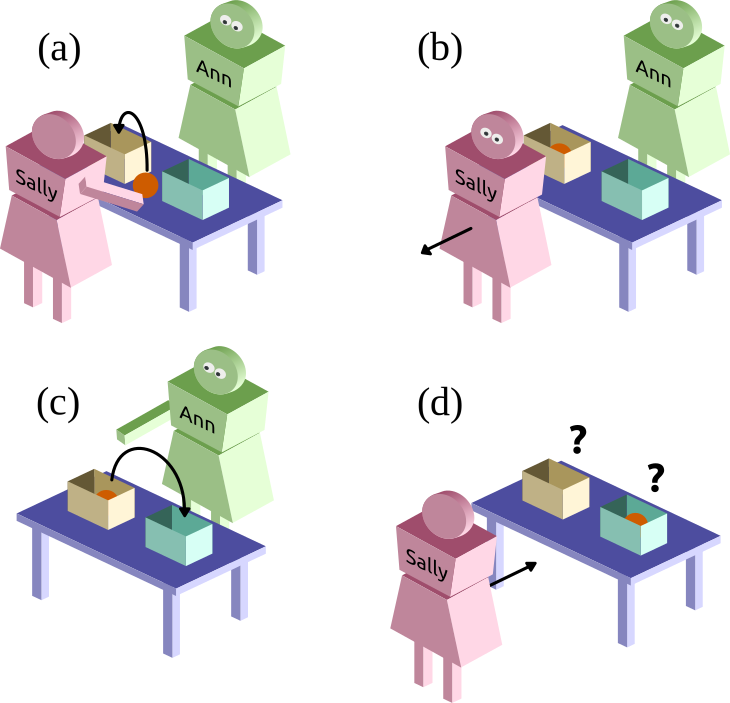
\includegraphics[width=0.7\linewidth]{sally_ann}
        \caption{\small The false belief experiment: two puppets, ``Anne'' and
            ``Sally'' face each other, with two boxes between them. A child (the
            subject) observes. Sally puts a ball in the beige box and then leaves.
            While she is absent, Anne moves the ball to the blue box. Sally
            returns. The experimenter asks the child: \emph{Where Sally would look
            for the ball?} Without a theory of mind, the child is not able
            to ascribe false beliefs to Sally, and therefore incorrectly answers
            \emph{In the blue box}. Visual perspective taking only is sufficient
            to pass this task.}

        \label{false-beliefs}
\end{figure}

Based on perspective taking \emph{Level 1} alone, Breazeal
\etal\cite{breazeal2009embodied} and Warnier \etal\cite{warnier2012when}
successfully tackled the classical hallmark of theory of mind, the false belief
experiment (Figure~\ref{false-beliefs}, introduced by~\cite{wimmer1983beliefs},
original experimental setting by~\cite{baron1985does}). They demonstrated
complete human-robot interaction scenarios where robots recognize and handle
false belief situations in dyadic or triadic interactions, and exhibit helping
behaviours that account for the missing/false beliefs of the human partners.

Those are significant achievements, also reassuring as to endow our robots with
advanced socio-cognitive capabilities.  However, one intuitively recognizes that
\emph{mutual modelling} goes indeed beyond computing what the human sees or does
not see. Perceptions translate into subjective representations: how can we
access them? How to measure what the other know about oneself? Many levels of
reciprocal modelling overlap, with endless ``I know that you know that I know
that...'': how to represent and manipulate them? What about the breadth of the
models we build?  Local to a given task or broader, deeper? How to tell apart
mimicry from cognitive modelling in a joint action?  Those many questions
underline the complexity of a cognitive mechanism that lays at the crossroad of
several academic fields. And robotics, as the science of embodied artifical
intelligence, may be a convergence point to validate our understanding of this
socio-cognitive skill.

This article contributes to this endavour by proposing a broad overview of
mutual modelling from four different perspectives in four different academic
domains. \emph{Developmental psychology} (and in particular developmental
\emph{patho}psychology), first, provides deep insights on human cognition and an
extensive experimental framework that has a strong potential in robotics.
\emph{Psycho-linguistic} and \emph{Collaborative Learning}, then, propose
concepts and tools to apprehend the importance and the dynamics of knowledge
sharing during social interactions. Third, we present the recent advancements in
\emph{cognitive neurosciences} that not only ground and shed light on the
physical mechanisms at stake when we model to other, but also provide original
experimental setups that may prove effective in robotics. Finally, we give a
look at the philosophy of the mind and the logical tools of \emph{formal
epistemology}: their use of modal logics to describe complex knowledge
manipulation in groups is likely a rewarding direction for robotics to explore.

\fixme{...
To prevent this article to be a ``catch-all'' of ...
Conceptual connections between these fields are numerous, we try to underline
them}

\section{Mutual Modelling and Developmental Psychology}

\paragraph{Connections vs. representations}

In~\cite{flavell1990developmental}, Flavell relates perspective taking
\emph{Level 1} to establishing \emph{cognitive connections} (I see, I hear, I
want, I like, I fear...), in contrast to perspective taking \emph{Level 2} that
relates to manipulating \emph{representations}.  This is exemplified by the
\emph{appearance-reality} tasks, like the \emph{elephant mask} experiment
proposed in~\cite{flavell1990developmental}: 3-years old children are not able
to tell that an experimenter hidden behind a large elephant mask but who speaks
normally \emph{looks} like an elephant, \emph{sounds} like the experimenter, and
\emph{really is} the experimenter.  It appears that, while children before 4
years are able to explicitly manipulate cognitive connections (they know for
instance that these are largely independent of each other and that they can
evolve over time) and know as well that their own connections are independent of
those of other people, they do not think that one concept can \emph{seriously}
(\ie, non playfully) hold several, possibly conflicting, representations.

This \emph{connection-representation} account appears to be an significant
component of a general theory of mind (one need to recognize that the same
object/concept may have different, serious, representations to then accept false
beliefs for instance),

%and, from an artificial intelligence perspective, raises
%an interesting challenge: how to design a meta-representational system
%that supports and manipulates multiple cognitive connections \emph{and}
%representations?

\begin{figure}
        \centering
        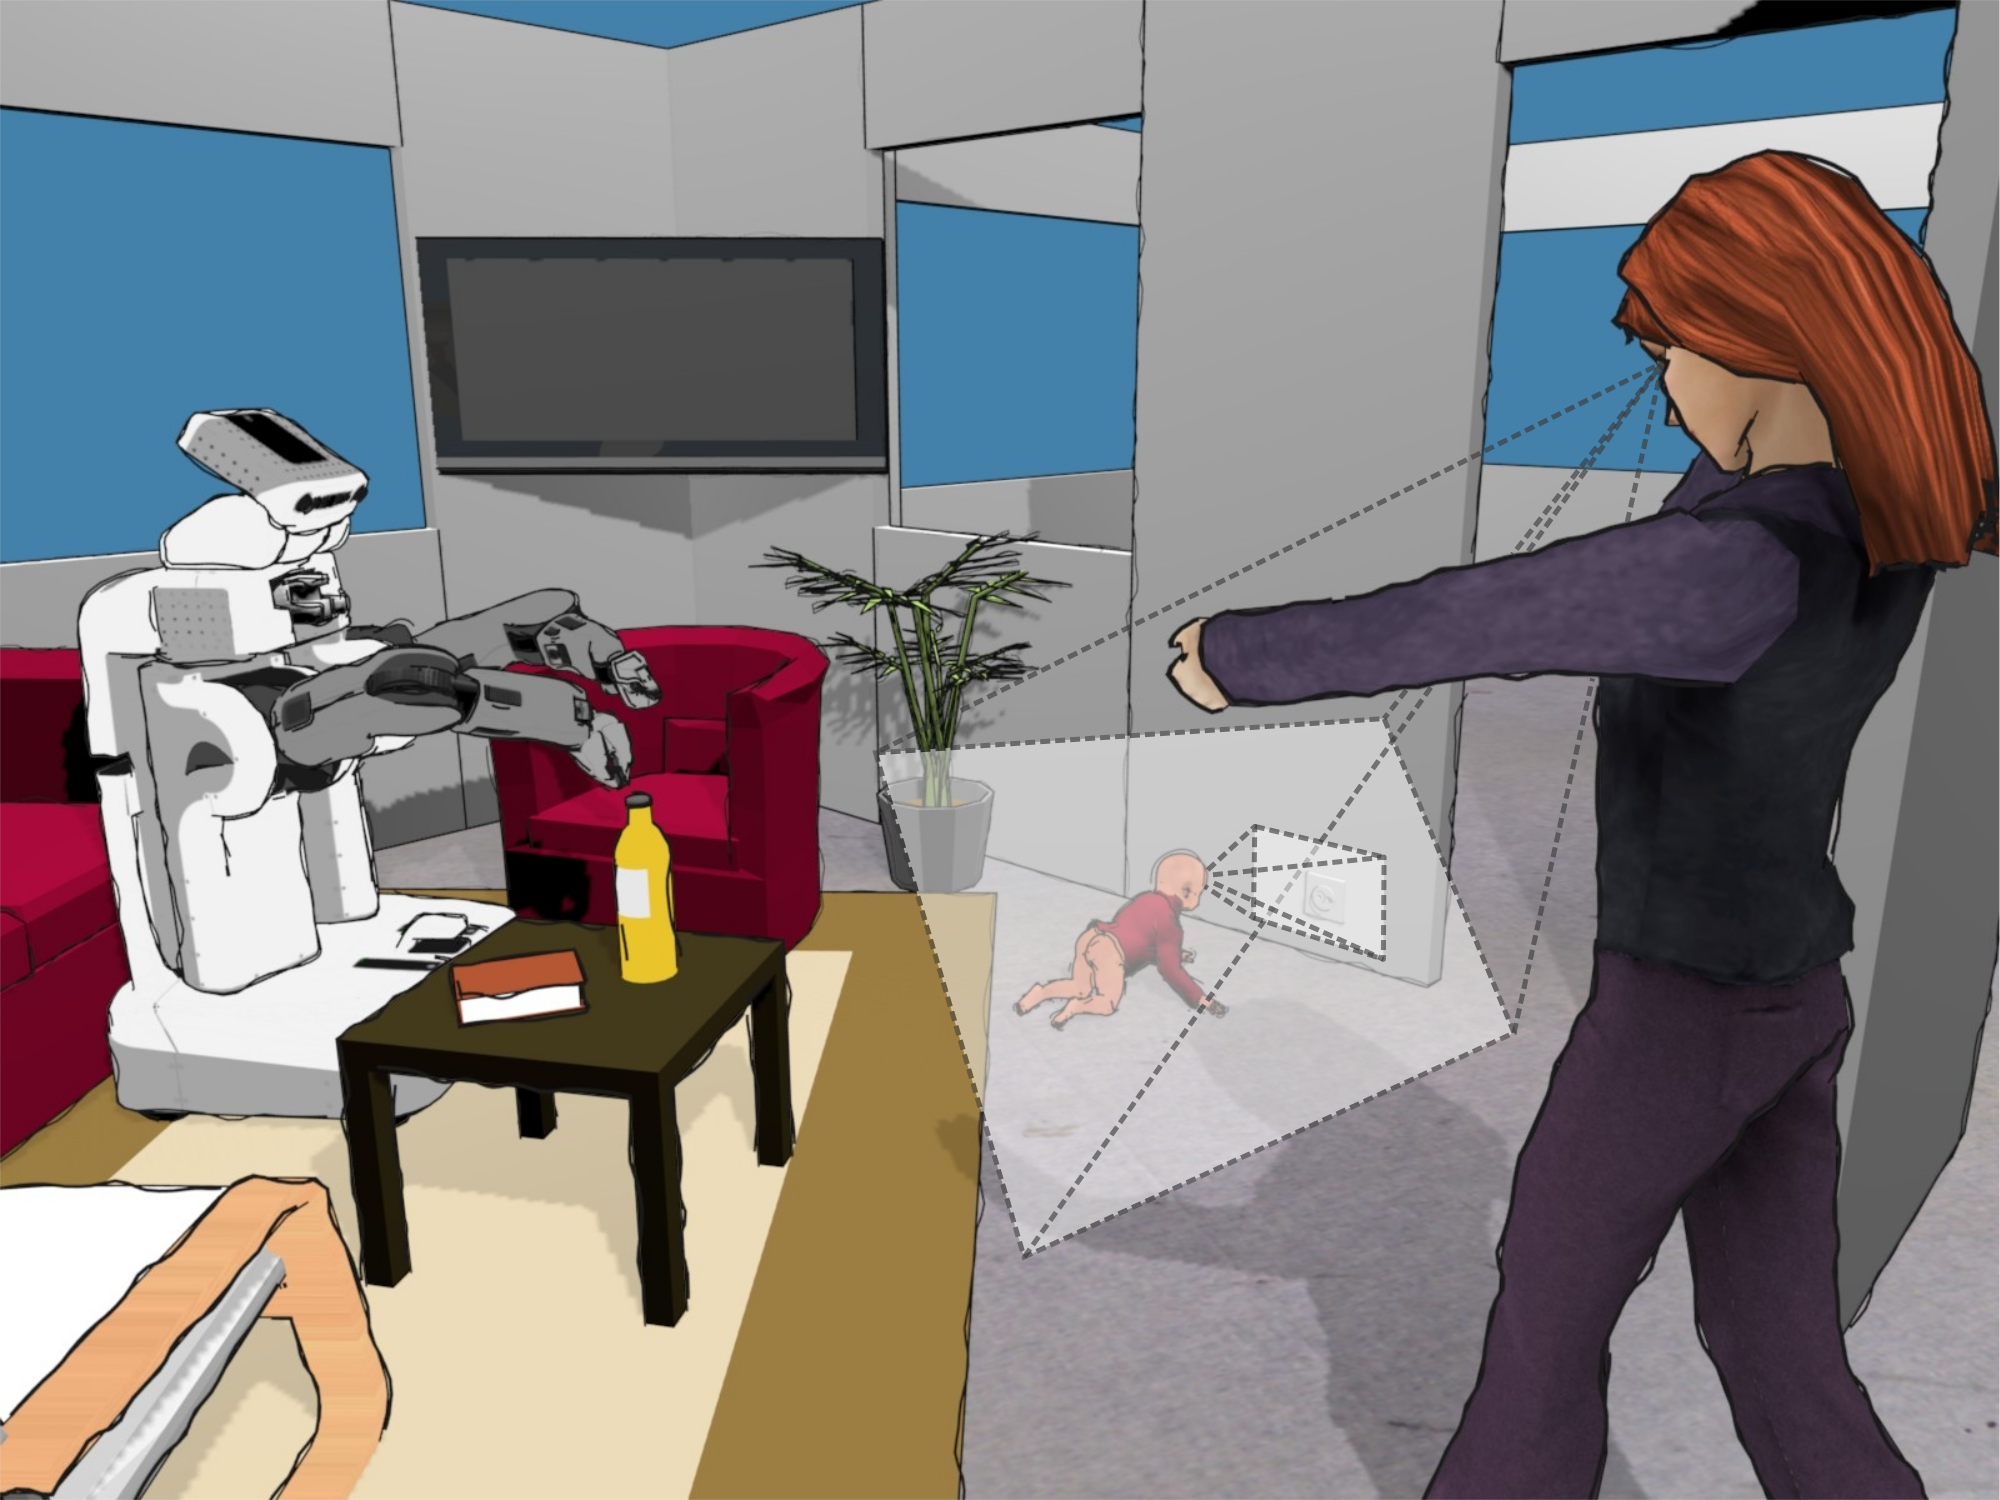
\includegraphics[width=0.9\columnwidth]{representation-perspective-taking}
        \caption{\small \emph{Visual} perspectives allow for a first level of mutual
            modelling. However, to correctly comprehend the scene,
            \emph{representation-level} perspective taking is required: what
            does the power socket means to the baby, what does the situation
            means to the mother.}

        \label{representation-level}
\end{figure}

Figure~\ref{representation-level} illustrates this difference between cognitive
connections and representations in an imaginary human-robot interaction
scenario. The \emph{visual} perspective of the baby and the mother are
represented: a robot endowed with perspective-taking level 1 is able to compute
that the baby looks at the plug and the mother looks at the baby.
\emph{Representation}-level perspective taking, on the other hand, would require
the robot to represent what the socket means to the baby (an attractive
affordance), and what the baby's behaviour represents to the mother (a potential
danger).


Incidentally, the false belief experiment was proposed by Baron-Cohen in the
frame of his research on autism (he shows that autistic children seem to
actually lack a theory of mind and suggests this as the primary cause of their
social impairments), and Frith and Happé further note in ~\cite{frith1994autism}
that this specific deficit of autism has led to a large amount of research which
proved, in turn, highly beneficial to the study of the development of theory of
mind in general. They reference in~\cite{frith1994autism} 13 such tasks, identified during
the study of social cognition by autistic children. Each of them is proposed in
two versions: one does not require mentalizing, while the other does require it.
One of these tasks, for example, required children to distinguish emotions,
namely happy/sad faces on one hand (situation-based emotion), and surprised
faces on the other (belief-based emotion)~\cite{baron1993children}.  Another
task, based on the \emph{penny-hiding game}, contrasts the two conditions in
terms of \emph{object occlusion} vs.~\emph{information
occlusion}~\cite{baron1992out} (we detail it hereafter). These tasks prototypically illustrate social
meta-cognition: one need to represent and reflect on someone else
representations (and not only perceptions), and they are not addressed by
today's research on social robots.

When reading literature on experimental research on autism, the apparent
simplicity of the proposed protocols often striking. This experimental research
is especially relevant to robotics because of the careful choice of interaction
modalities: since autistic children frequently exhibit impairments beyond social
ones (such as motor or linguistic ones), the experiments must be designed such
that they require only basic cognitive skills besides the social abilities that
are tested. The Sally and Anne task, for instance, requires the observing child
to be able to visually follow the marble, to remember the true location of the
marble, to understand simple questions (``Where will Sally look for her
marble?'' in Baron-Cohen's protocol~\cite{baron1985does}) and eventually to give
an answer, either verbally or with a gesture. The two first premises are
actually explicitely checked through questions: ``Where is the
marble really?'' -- reality question -- and ``Where was the marble in the
beginning?'' -- memory question.

Likewise, current social robots have limited cognitive skills (no fast yet fine
motor skills, limited speech production and understanding, limited scene
segmentation and object recognition capabilities, etc.) and such tasks
that effectively test a single cognitive skill (in this case, mentalizing) in
near isolation are of high interest for experimental social robotics.

Frith and Happé have listed in~\cite{frith1994autism} eight tasks
(Table~\ref{mentalizing-tasks} reproduces this list) that have been
used in the literature to evidence the presence or absence of a theory of mind
by children. This list is interesting in that it mirrors pairs of tasks: ones
which do not require mentalizing with similar ones which do require mentalizing,
thus providing control tasks.

\begin{table}[h]
    \centering
    \begin{tabular}{p{0.4\linewidth}p{0.5\linewidth}}
        \toprule
        No mentalizing required           & Mentalizing required          \\
        \midrule
        Ordering behavioural pictures     & Ordering mentalistic pictures~\cite{baron1986mechanical} \\
        Understanding see                 & Understanding know~\cite{perner1989exploration}            \\
        Protoimperative pointing          & Protodeclarative pointing~\cite{baron1989perceptual}     \\
        Sabotage                          & Deception~\cite{sodian1992deception}                     \\
        False photographs                 & False beliefs~\cite{leslie1992domain}                 \\
        Recognizing happiness and sadness & Recognizing surprise~\cite{baron1993children}          \\
        Object occlusion                  & Information occlusion~\cite{baron1992out}         \\
        Literal expression                & Metaphorical expression~\cite{happe1993communicative}       \\
        \bottomrule
    \end{tabular}
    \caption{\small Tasks requiring or not mentalizing to pass, listed by Frith and Happé in~\cite{frith1994autism}}
    \label{mentalizing-tasks}
\end{table}

\emph{Object occlusion} vs.~\emph{Information occlusion} is one example of a
(pair of) task(s) which evidence representation-level perspective taking through
adaptive deception: during a simple game, the experimenter adapts its strategy
(deceptive/non-deceptive behaviour) to the representation skills of its child
opponent. The experimental setting is derived from the penny-hiding game
protocol originally proposed by Oswald and Ollendick~\cite{oswald1989role} and
replicated and extended by Baron-Cohen in~\cite{baron1992out}, who describes it
as a two-person game in which the subject is actively involved, either as a
guesser or as a hider. The hider hides the penny in one hand or the other, and
then invites a guess. The game is repeated several time before switching the
roles. Baron-Cohen proposes a specific index to rate the level of the players
based on the idea of \emph{information occlusion}: minimally, the hider must
ensure \emph{object occlusion} (the penny must not become visible to the
guesser), while good hiders, with representation-level perspective taking
skills, develop strategies (like random hand switching or deictic hints at the
wrong hand) to prevent the guesser to find the penny (\emph{information
occlusion}). One could imagine a similar protocol adapted to robotics: the robot
would for instance play the role of the experimenter, adapting on-line its
behaviour to what it understands of the perspective taking capabilities of the
children, and would consequently require \emph{second-order},
\emph{representation-level} perspective taking from the robot.



\paragraph{Higer-order Theory of Mind}

While a great deal of research concerns itself with \emph{first-order} theory of
mind, \emph{higher-order} (and particularly, second-order) ToM are also studied.
Verbrugge and Mol~\cite{verbrugge2008learning} describe the different levels in
the following terms:
\begin{quote}
To have a first-order ToM is to assume that someone's beliefs, thoughts and
desires influence one's behavior. A first-order thought could be: \emph{He does not
know that his book is on the table}. In second-order ToM it is also recognized
that to predict others' behavior, the desires and beliefs that they have of
one's self and the predictions of oneself by others must be taken into account.
So, for example, you can realize that what someone expects you to do will affect
his behavior. For example, ``(I know) he does not know that I know his book is on
the table'' would be part of my second-order ToM. To have a third-order ToM is to
assume others to have a second-order ToM, etc.
\end{quote}

Flobbe \etal propose in~\cite{flobbe2008children} a set of three tasks (a
second-order false belief task, a strategic game and a sentence comprehension
test) that require second-order mentalizing to succeed.\fixme{present the
chocolate bar task}

Agreement is understood later than 2nd order ToM because it's recursive.
\cite[p.~664]{verbrugge2009logic}.

\paragraph{Pretense}

a second direction for the 'meta-cognitive foundations of mind modelling' is
Leslie's paper on the role of pretense []. I still need to investigate it

\fixme{another paper of high relevance is by Frye et al. []: they use a computational
metaphor to approach theory of mind, contrasting here also
rule-based tasks with tasks requiring a theory of mind. I also need to
investigate it further. For the formal epistemology section?}

\fixme{Limits of ToM:
\cite{keysar2003limits}: adults, even with working theory of mind, may prefer
their own perspective and ignore the other perspective.}


\section{Mutual Modelling in Psycholinguistics and Collaborative Learning}

\paragraph{Mutual modelling as a support for shared understanding}

\emph{Computer Supported Collaborative Learning} (CSCL) researches the cognitive
mechanisms and practical techniques underpinning efficient learning in social
situations. From its very beginning, CSCL research has been following
Roschelle and Teasley suggestion~\cite{roschelle1995construction} that
collaborative learning has something to do with the process of constructing and
maintaining a \emph{shared understanding} of the task at hand. Building a shared/mutual
understanding refers to the upper class of collaborative learning situations,
those in which students should build upon each other's understanding to refine
their own understanding.  What is expected to produce learning is not the mere
fact that two students build the same understanding but the cognitive effort
they have to engage to build this shared
understanding~\cite{schwartz1995emergence}.

The construction of a shared understanding has been investigated for several
years in psycholinguistics, under the  notion of ``grounding''\footnote{Note
that the meaning of \emph{grounding} -- ensuring a shared understanding of a
situation during an interaction -- that we employ in this article must be
distinguished from its meaning in the context of \emph{symbol grounding} as
defined by Harnad~\cite{harnad1990symbol}}~(Clark,
in~\cite{clark1986referring}).  However, the relevance of grounding mechanisms
for explaining learning outcomes has been questioned in learning sciences. The
monitoring and repair of mis-understanding explains for instance referential
failures in short dialogue episodes but does hardly predict \emph{conceptual
change} (\ie the acquisition, acceptation and integration into one's mental
model of a new belief\fixme{check with Pierre}) over longer
sessions~\cite{dillenbourg2006sharing}. The cumulative effect of grounding
episodes can probably be better understood from a socio-cultural perspective:
\emph{``collaborative learning is associated with the increased
cognitive-interactional effort involved in the transition from learning to
understand each other to learning to understand the meanings of the semiotic
tools that constitute the mediators of interpersonal
interaction''}~\cite{baker1999role}\fixme{Ask Pierre for explanations}, and
several scholars suggest that CSCL research should go deeper in the
understanding of how partners engage into shared meaning
making~\cite{stahl2007meaning} or \emph{intersubjective} meaning
making~\cite{suthers2006technology}.

Paradoxically, while Clark's theory is somewhat too linguistic from a conceptual
change viewpoint, it is criticized at the same time as being too cognitivist by
some psycholinguists, \ie as overestimating the amount of shared knowledge and
mutual representations actually necessary to conduct a dialogue. The fundamental
issue, as old as philosophy, is the degree of coupling between the different
levels of dialogue, mostly between the lexical/syntactical level and the deeper
semantic levels. In~\cite{pickering2006alignment}, Pickering and Garrod argue
that the mutual understanding starts mostly with a \emph{superficial alignment}
at the level of the linguistic representations, due to priming mechanisms, and
that this local alignment may -- in some cases -- lead to a \emph{global
alignment} of the semantic level (\emph{deep grounding}).  For these authors,
the convergence in dialogue, and even the repair of some misunderstandings, is
explained by this mimetic behavior more than by a monitoring of each other's
knowledge: \emph{``...interlocutors do not need to monitor and develop full common
ground as a regular, constant part of routine conversation, as it would be
unnecessary and far too costly. Establishment of full common ground is, we
argue, a specialized and non-automatic process that is used primarily in times
of difficulty (when radical misalignment becomes
apparent).''}~\cite{pickering2006alignment} This view is
actually not incompatible with Clark's \emph{grounding
criterion}~\cite{clark1989contributing}: the degree of shared understanding that
peers need to reach depends upon the task they perform. For instance, a dialogue
between two surgeons might rely on superficial alignment if they talk about
their friends but has to guarantee accurate common grounds when talking about
which intervention will be conducted in which way on which patient.

%This interesting cognitive science debate mostly occurred outside the field of
%learning science. In education, the question is to relate these mechanisms to
%learning outcomes. Is linguistic alignment sufficient to trigger conceptual
%change? Does negotiation of meaning only occurs when partners monitor and
%diagnose each other's knowledge. If the ratio between shallow alignment and deep
%grounding depends upon the task, and if deep grounding is a condition for
%learning, then the pedagogical challenge is to design tasks that require deep
%grounding. Most empirical studies on grounding and alignment are conducted with
%tasks, which despite being qualified as ``ecologically valid'' by their authors,
%are mere referencing tasks such as asking the way to the train station or
%helping the peer to choose a picture among many. In this contribution, we
%explore several richer tasks such as arguing on a sensitive issue or building a
%concept map.

Deep grounding or shared meaning making requires some cognitive load. For Clark,
what is important is not the individual effort made by the receiver of a
communicative act, but the overall \emph{least collaborative
effort}~\cite{clark1986referring}.  The cost of producing a perfect utterance
may be higher than the cost of repairing the problems that may arise through
misunderstandings. For instance, subjects are less careful about adapting their
utterances to their partner when they know they can provide feedback on his/her
understanding~\cite{schober1993spatial}. Dillenbourg \etal introduced the
notion of \emph{optimal collaborative effort}~\cite{dillenbourg1995evolution} to
stress that misunderstanding should not be viewed as something to be avoided (if
this was possible), but as an opportunity to engage into verbalization,
explanation, negotiation, and so forth.

\paragraph{CSCL model of mutual modelling}
\label{cscl-model}

Dillenbourg proposes in~\cite{sangin2007partner} a model to represent mutual
modelling situations. He uses the notation \model{A}{B}{X} to denote ``$A$ knows
that $B$ knows $X$'' (equivalent to the epistemic logic notation
$\mathsf{K}_{A}\mathsf{K}_{B}X$ that we present in the next section). This
notation does not mean $A$ has an explicit, monolithic representation of $B$: it
must be understood as an abstraction referring to complex socio-cognitive
processes. Besides, he refer to the \emph{degree of accuracy} of the model as
\Model{A}{B}{X}.

He parametrizes and assesses the mutual modelling effort through 3 variables:

\begin{enumerate}

    \item Tasks vary a lot with respect to how much they require mutual
        understanding.  The \emph{grounding criterion}~\cite{clark1986referring}
        \groundingcriterion refers to
        how important it is to mutually share a piece of information $X$ to
        succeed the task $T$. It can be computed as the probability to succeed $T$
        despite the fact $X$ is not grounded. $\mathcal{M}^{\circ}_{min}(A,B,X)$
        can be estimated from the correlation between \Model{A}{B}{X} and task
        performance. 

    \item Before any specific grounding action, there is usually a non-null
        probability that $X$ is mutually understood by $A$ and $B$ (\eg $X$
        is part of $A$'s and $B$'s cultures, it is manifest to co-present
        subjects or simply there is not much space for misunderstanding
        or disagreement about $X$). He note the theoretical accuracy of
        initial grounds $\mathcal{M}^{\circ}_{t_0}(A,B,X)$.

    \item The cost of grounding $X$ refers to the physical and cognitive effort
        required to perform a grounding act $\alpha$: a verbal repair (\eg
        rephrasing), a deictic gesture, a physical move to adopt one partner's
        viewpoint, etc. This cost varies according to media
        features~\cite{clark1991grounding}.

\end{enumerate}

These notations lead to simple representations of mutual modelling during
interactions, and Dillenbourg derives several questions out of this model.
Adapted to a human-robot interaction situation, Figure~\ref{mm_symmetry}
represents for instance a dyadic interaction (we hereafter use $H$ to denote a
human, while $R$ stands for a robot). $\Delta_1$ illustrates what Dillenbourg
calls the \emph{symmetry} question ({\it is the accuracy of my model related or
not to the accuracy of your model?}).

\begin{figure}[htb]
\centering

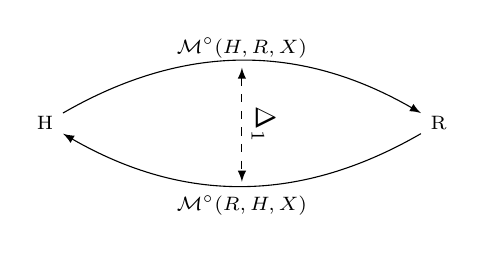
\begin{tikzpicture}[>=latex, scale=0.5]

\draw(0,0) node[anchor=north] (A) {\scriptsize H};
\draw(10,0) node[anchor=north] (B) {\scriptsize R};
\draw(5,2) node[anchor=north] {\scriptsize \Model{H}{R}{ X}};
\draw(5,-2) node[anchor=north] {\scriptsize \Model{R}{H}{ X}};
\draw[dashed, <->] (5,1) -- (5,-1.9) node[midway, sloped, above] {$\Delta_1$};
\draw[->] (A) to[bend left] (B);
\draw[->] (B) to[bend left] (A);

\end{tikzpicture}

\caption{\small Mutual modelling in a dyadic interaction, $\Delta_1 =
    \Delta(\mathcal{M}^{\circ} (H,R,X),
\mathcal{M}^{\circ} (R,H,X))$}

\label{mm_symmetry}
\end{figure}


With triads (two humans $H_1$ and $H_2$ and a robot $R$), we may compute the
accuracy of 6 models \Model{H_1}{H_2}{X}, \Model{H_2}{H_1}{X},
\Model{H_1}{R}{X}, \Model{R}{H_1}{X}, \Model{R}{H_2}{X} and \Model{H_2}{R}{X}.

This leads to two \emph{triangle questions} relevant ot HRI (Figure~\ref{mm_triangles}): Do $H_1$ and $H_2$ have the same
accuracy when modelling the robot $R$? ($\Delta_2 = \Delta(\M{H_1}{R}{X},
\M{H_2}{R}{X})$), and conversely, what may lead $R$ to model more accurately
$H_1$ or $H_2$? ($\Delta_3 = \Delta(\M{R}{H_1}{X}, \M{R}{H_2}{X})$).


\begin{figure}[htb]
\centering
\subcaptionbox{}{ 
    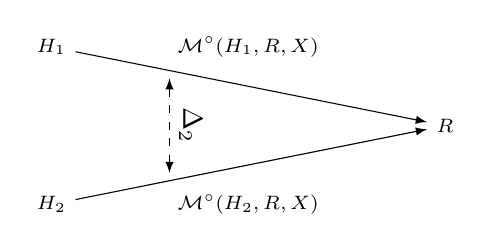
\begin{tikzpicture}[>=latex, scale=0.5]

    \draw(0,2) node (A) {\scriptsize $H_1$};
    \draw(0,-2) node (B) {\scriptsize $H_2$};
    \draw(10,0) node (C) {\scriptsize $R$};

    \draw(5,2) node {\scriptsize \Model{H_1}{ R}{ X}};
    \draw(5,-2) node {\scriptsize \Model{H_2}{ R}{ X}};
    \draw[dashed, <->] (3,1.2) -- (3,-1.2) node[midway, sloped, above] {$\Delta_2$};
    \draw[->] (A) to (C);
    \draw[->] (B) to (C);

    \end{tikzpicture}
}
\subcaptionbox{}{ 
    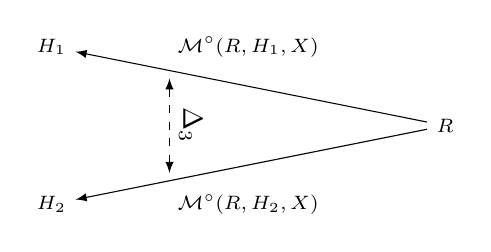
\begin{tikzpicture}[>=latex, scale=0.5]

    \draw(0,2) node (A) {\scriptsize $H_1$};
    \draw(0,-2) node (B) {\scriptsize $H_2$};
    \draw(10,0) node (C) {\scriptsize $R$};

    \draw(5,2) node {\scriptsize \Model{R}{ H_1}{ X}};
    \draw(5,-2) node {\scriptsize \Model{R}{ H_2}{ X}};
    \draw[dashed, <->] (3,1.2) -- (3,-1.2) node[midway, sloped, above]
    {$\Delta_3$};
    \draw[<-] (A) to (C);
    \draw[<-] (B) to (C);

    \end{tikzpicture}
}
\caption{\small Mutual modelling in a triadic interaction}

\label{mm_triangles}
\end{figure}

Finally, Dillenbourg also suggests a \emph{rectangle question}: how self- versus
other modelling compares ($\Delta_4$ in Figure~\ref{mm_rectangle})? This gives
an indication of meta-cognitive skills of the agents. We can also question if
the modelling skills depend upon what aspects are being modeled ($X$ or $Y$)
which would explain vertical differences ($\Delta_5$ in
Figure~\ref{mm_rectangle}).

\begin{figure}[htb]
\centering

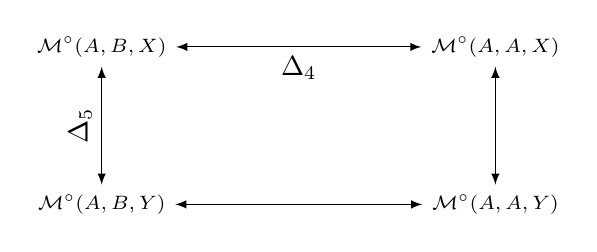
\begin{tikzpicture}[>=latex, scale=0.5]

    \draw(0,0) node (a) {\scriptsize \Model{A}{ B}{ X}};
    \draw(10,0) node (b) {\scriptsize \Model{A}{ A}{ X}};
    \draw(10,-4) node (c) {\scriptsize \Model{A}{ A}{ Y}};
    \draw(0,-4) node (d) {\scriptsize \Model{A}{ B}{ Y}};
    \draw[<->] (a) -- (b) node[midway, below] {$\Delta_4$};
    \draw[<->] (b) -- (c);
    \draw[<->] (c) -- (d);
    \draw[<->] (d) -- (a) node[midway, sloped, above] {$\Delta_5$};

\end{tikzpicture}

\caption{\small Meta-cognitive skills and domain-dependent modelling}

\label{mm_rectangle}
\end{figure}

This model, designed in the context of human collaboration, 
evidences questions that are relevant as well to human-robot interactions.

%
%\begin{figure}
%        \centering
%        \setlength{\columnsep}{0.1cm}
%        \begin{multicols}{2}
%            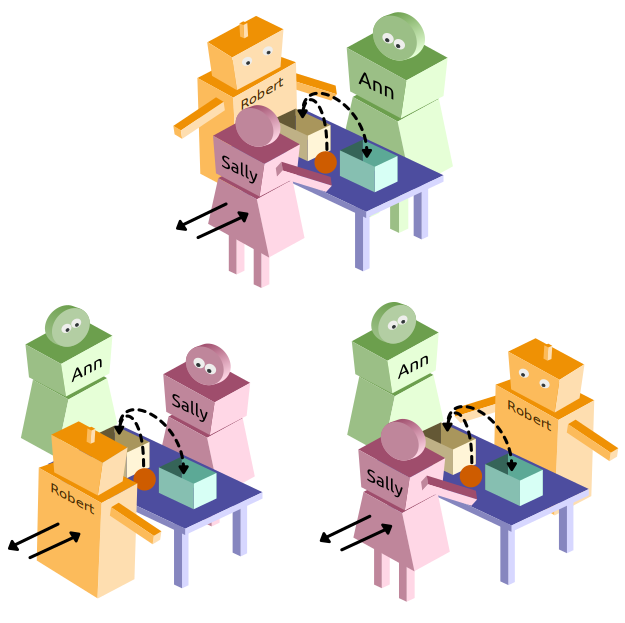
\includegraphics[width=1.0\columnwidth]{triadic_false_beliefs.pdf}
%
%            \resizebox{\columnwidth}{!}{
%            \begin{tikzpicture}[
%                    >=latex,
%                scale=0.5]
%
%                \draw(0,2) node (A) {\scriptsize Sally};
%                \draw(0,-2) node (B) {\scriptsize Ann};
%                \draw(10,0) node (C) {\scriptsize robot};
%
%                \draw(5,2) node {\scriptsize \Model{Sally}{ R}{ X}};
%                \draw(5,-2) node {\scriptsize \Model{Ann}{ R}{ X}};
%                \draw[dashed, <->] (3,1.2) -- (3,-1.2) node[midway, sloped, above] {$\Delta_2$};
%                \draw[->,very thick] (A) to (C);
%                \draw[->,very thick] (B) to (C);
%
%
%                \draw(0,-4) node (A) {\scriptsize Sally};
%                \draw(0,-8) node (B) {\scriptsize Ann};
%                \draw(10,-6) node (C) {\scriptsize robot};
%
%                \draw(5,-4) node {\scriptsize \Model{R}{ Sally}{ X}};
%                \draw(5,-8) node {\scriptsize \Model{R}{ Ann}{ X}};
%                \draw[dashed, <->] (3,-5.2) -- (3,-7.2) node[midway, sloped, above]
%                {$\Delta_3$};
%                \draw[<-,very thick] (A) to (C);
%                \draw[<-,very thick] (B) to (C);
%
%            \end{tikzpicture}
%            }
%        \end{multicols}
%
%    \caption{blabla}
%    \label{}
%\end{figure}

\fixme{Discuss experimental settings in CSCL?}

\section{Mutual Modelling in Neurosciences}

\begin{itemize}
    \item models?
    \item experimental methodologies/settings?
\end{itemize}


\section{Formal Epistemology}
\label{formal-epistemology}

\emph{Modal logics} look at the formal representation of \emph{possible
worlds}, \ie the \emph{possibility} or \emph{necessity} of certain assertions
to hold, and is naturally suited to build mathematical representations of
situations such as ``\emph{the robot knows (the baby may not know what a power
socket is)}''.

The \emph{epistemic modal logic} (see~\cite{hendricks2008epistemic} for an
overview and references), in particular, focuses on the formal representation of
knowledge and beliefs of agents, with the operators $\mathsf{K}_{i}\varphi$
(epistemic operator: agent $i$ knows $\varphi$) and $\mathsf{B}_{i}\varphi$
(doxatic operator: agent $i$ believes $\varphi$). Every possible logical
propositions belong then to possible \emph{worlds} (noted $w$), that are
\emph{accessible} (\ie compatible) or not to one's beliefs and knowledge.

Single-agent epistemic systems can naturally extend to multi-agent systems~\cite[chapt.
4]{fagin1995reasoning}: if $p$ stands for ``the power socket is dangerous'',
$\mathsf{K}_{mother}p \wedge \mathsf{K}_{mother}\neg\mathsf{K}_{baby}p$ states
that the mother knows that the socket is dangerous, and also knows that the baby
is not aware of this. This provides a formal tool to represent mutual models
(the \emph{order} of mutual modelling as discussed in the context of
developmental psychology is here directly
related to the nesting depth of the epistemic operator).

This approach has led to applications to the representation of knowledge
dynamics on concrete, ableit arguably toy, scenarios: van Ditmarsch presents for
instance in~\cite{ditmarsch2002description} the formal description of possible
Cluedo strategies based on what players know about other players' knowledge;
Verbrugge and Mol analyse mutual modelling in a strategic game with imperfect
information (derived from Mastermind) in~\cite{verbrugge2008learning}.

Verbrugge further investigates the social aspect of epistemic logics
in~\cite{verbrugge2009logic} and proposes a survey of epistemic logic
applications to \emph{social reasoning}. He underlines both the limits of
epistemic logic for that purpose (the common epistemic systems $\mathbf{S4}$ and
$\mathbf{S5}$ assume for instance $\mathsf{K}_{i}\varphi \rightarrow
\mathsf{K}_{i}\mathsf{K}_{i}\varphi$, which reads ``$i$ knows $\varphi$''
implies ``$i$ knows that $i$ knows $\varphi$'', \ie $i$ can always introspect, a
rather idealized model of human cognition) and the recent advancement towards
modeling \emph{human} social cognition, which implies for instance limited
rationality.  One of these attempts is formalized as a \emph{doxastic epistemic
logic} by van Ditmarsch and Labuschagne in~\cite{ditmarsch2007beliefs}, with an
explicit focus on modeling \emph{theory of mind} mechanisms. This model builds
upon \emph{dynamic epistemic logic}~\cite{ditmarsch2007dynamic} (DEL, epistemic
logics augmented with mechanisms for knowledge changes), and the
modelling of agents' degrees of belief through a \emph{preference} accessibility
relation.

The mathematical objects build from these different modal logics, are natural
candidates for transposition into representational systems and controllers for
robots. Historically in robotics, the main research perspective has been towards
the \emph{action logics}, and in particular the influential \emph{situation
calculus} (a propositional logic initially proposed by McCarthy, and fully
axiomatized in the context of robotics by Levesque \etal
in~\cite{levesque1998foundations}, which led to the {\sc golog} logic
programming language~\cite{levesque1997golog}).  Many other action logics have
been proposed including modal logics like PDL (\emph{Propositional Dynamic
Logic}).

Recent efforts have focused on bridging action logics (that deal with
\emph{ontic} actions, \ie actions which have tangible, physical consequences)
with epistemic logics (that deal with \emph{epistemic} actions, \ie knowledge
changes). Van Ditmarsch proposes in~\cite{ditmarsch2010from} for instance a
solution to embed a practical subset of situation calculus into a dynamic
epistemic logic, and Herzig provides in~\cite{herzig2014logics} a broader
overview of the interplay between current action and epistemic logics.

From a practical perspective however, implementations of these logics into
practical reasoners or programming languages remain rare. The development of
\emph{Description Logics} (DL) in the knowledge representation community, along
with effective, practical tools (like reasoners) is a possible path forward,
since DL semantics overlap to some extend with modal logics~\cite[chap.
4.2.2]{baader2003description}, and \emph{Description Logics} have already been
successfully used in robotics (see~\cite{lemaignan2012symbolic} for a review).


\section{Conclusion: Towards socio-cognitive robotics}

Several lessons can be taken out of these four perspectives on mutual modelling.
First, \textbf{concepts} and terminology stand out and social robotics would
benefit of incorporating them. Second, \textbf{models} of mutual modelling exist
that would make sense in robotics as well, along with investigation strategies
and approaches that translate well to robotics. Finally, we believe that several
\textbf{experimental settings} designed and successfully tested in other
disciplines shape an interesting way forward for (experimental) social robotics.

\subsection{Concepts}

Several concepts have been introduced that help with decomposing the broad idea
of mutual modelling into better delimited research questions.

Flavell's distinction between \emph{cognitive connections} on one hand, and
\emph{mental representation} on the other hand helps for instance in recognizing
the limits of perceptual perspective taking as currently achieved in robotics.
And from an artificial intelligence perspective, this
\emph{connection-representation} account indeed raises an interesting challenge:
how to design a meta-representational system that supports and manipulates
multiple cognitive connections \emph{and} representations?

\emph{Modelling order}: 2nd order around 8~\cite{perner1988higher}

The level of mutual modelling required for effective collaboration is another
question that is relevant to human-robot interaction. Pickering and Garrod, with
the idea of \emph{superficial alignment} versus \emph{global alignment} or
\emph{deep grounding}, come to the conclusion that \emph{mimicking} behaviours
is often a more efficient way to work together than establishing a full common
ground, which is also expressed by Clark in terms of \emph{least collaborative
effort} and Dillenbourg in terms of \emph{optimal collaborative effort}:
misunderstandings should not be viewed as something to systematically avoid
since the repair actions they may elicit can also be viewed as a way to engage
the agents into new interactions. Clark and Dillenbourg developed this idea in
the context of collaborative learning (where social interactions are designed to
support learning), we believe it applies equally well to the context of
human-robot interaction.  In that respect, Clark's concept of \emph{grounding
criterion} provides a practical tool to represent and manipulate this idea of
degree of shared understanding required by the agents to perform a given task.

%%%%%%%%%%%%%%%%%%%%%%%%%%%%%%%%%%%%%%%%%%%%%%%%%%%%%%%%%%%%%%%%%%%%%%%%%%%%%%%%

% Hidden for double blind review
%\section*{Acknowledgments}
%
%This research was supported by the Swiss National Science Foundation through the
%National Centre of Competence in Research Robotics.


%%%%%%%%%%%%%%%%%%%%%%%%%%%%%%%%%%%%%%%%%%%%%%%%%%%%%%%%%%%%%%%%%%%%%%%%%%%%%%%%

%\begin{thebibliography}
\bibliographystyle{abbrv}
\bibliography{mutual-modelling}

%\end{thebibliography}

\end{document}
